\documentclass[14pt, fleqn, xcolor={dvipsnames, table}]{beamer}
\usepackage[T2A]{fontenc}
\usepackage[utf8]{inputenc}
\usepackage[english,russian]{babel}
\usepackage{amssymb,amsfonts,amsmath,mathtext}
\usepackage{cite,enumerate,float,indentfirst}
\usepackage{cancel}

\usepackage{tikz}                   
\usetikzlibrary{shadows}

% \usepackage{enumitem}
% \setitemize{label=\usebeamerfont*{itemize item}%
%   \usebeamercolor[fg]{itemize item}
%   \usebeamertemplate{itemize item}}

\graphicspath{{images/}}

\usetheme{Madrid}
\usecolortheme{seahorse}
\renewcommand{\CancelColor}{\color{red}}

\setbeamercolor{footline}{fg=Blue!50}
\setbeamertemplate{footline}{
  \leavevmode%
  \hbox{%
  \begin{beamercolorbox}[wd=.333333\paperwidth,ht=2.25ex,dp=1ex,center]{}%
    И. Кураленок, Н. Поваров, Яндекс
  \end{beamercolorbox}%
  \begin{beamercolorbox}[wd=.333333\paperwidth,ht=2.25ex,dp=1ex,center]{}%
    Санкт-Петербург, 2014
  \end{beamercolorbox}%
  \begin{beamercolorbox}[wd=.333333\paperwidth,ht=2.25ex,dp=1ex,right]{}%
  Стр. \insertframenumber{} из \inserttotalframenumber \hspace*{2ex}
  \end{beamercolorbox}}%
  \vskip0pt%
}
\newcommand\indentdisplays[1]{%
     \everydisplay{\addtolength\displayindent{#1}%
     \addtolength\displaywidth{-#1}}}
\newcommand{\itemi}{\item[\checkmark]}

\title{Пару слов про сэмплирование\\\small{}}
\author[]{\small{%
И.~Куралёнок}}
\date{}

\begin{document}

\begin{frame}
\maketitle
\small
\begin{center}
\vspace{-60pt}
\vspace{80pt}
\footnotesize СПб, 2017
\end{center}
\end{frame}

% \begin{frame}{Содержание}
% \begin{enumerate}
%   \item Понятие сэмплирования
%   \begin{itemize}
%    \item Процесс сэмплирования
%    \item Основные методы сэмплирования
%   \end{itemize}
%   \item Переборные методы в ML
%   \begin{itemize}
%    \item Полный перебор
%   \end{itemize}
%   \item Hill climbing
%   \item Сэмплирование марковскими цепями
%   \begin{itemize}
%    \item Metropolis-Hastings алгоритм
%    \item Алгоритм Гиббса
%   \end{itemize}
%   \item Построение вероятностного пространства для максимизации
% \end{enumerate}
% \end{frame}

\section{Создание обучающей выборки}

\subsection{Сэмплирование}
\begin{frame}{Понятие сэмплирования}
\textit{Сэмплирование} --- метод исследования множества путём анализа его подмножеств. \\
Применяется когда:
\begin{itemize}
   \item множество слишком велико для перебора;
   \item каждое дополнительное измерение дорого;
   \item предварительный анализ.
\end{itemize}
\end{frame}

\begin{frame}{Алгоритм сэмплирования}
\begin{enumerate}
   \item Понять какое множество мы изучаем
   \item Осознать, что из этого множества мы можем измерить
   \item Определить количество измерений
   \item Разработать план сэмплирования
   \item Провести сэмплирование
\end{enumerate}
\end{frame}

\begin{frame}{Типы сэмплирования}
\begin{itemize}
   \item Вероятностное сэмплирование: 
   $$
   P(x),\forall x:P(x) > 0
   $$
   \uncover<2>{\textit{Например: попробуем посчитать соотношение мужчин/женщин}}
   \item Невероятностное сэмплирование:
   $$
   P(x), \exists x: P(x) = 0
   $$
   \uncover<3>{\textit{Например: ``по результатам опроса superjob.ru, 100\% россиян пользуются интернетом''}}
   \item Без возвращений
   \item С возвращениями
\end{itemize}
\end{frame}

\begin{frame}{Виды сэмплирования}
\begin{itemize}
   \item Вероятностное сэмплирование
   \begin{itemize}
    \item Простое вероятностное
    \item Систематическое
    \item Пропорциональное
    \item Кластерное
    \item Стратифицированное
   \end{itemize}
   \item Невероятностное сэмплирование
   \begin{itemize}
    \item Опрос ближайших
    \item Панельное сэмплирование
   \end{itemize}
\end{itemize}
\end{frame}

\begin{frame}{Простое вероятностное}
\begin{center}
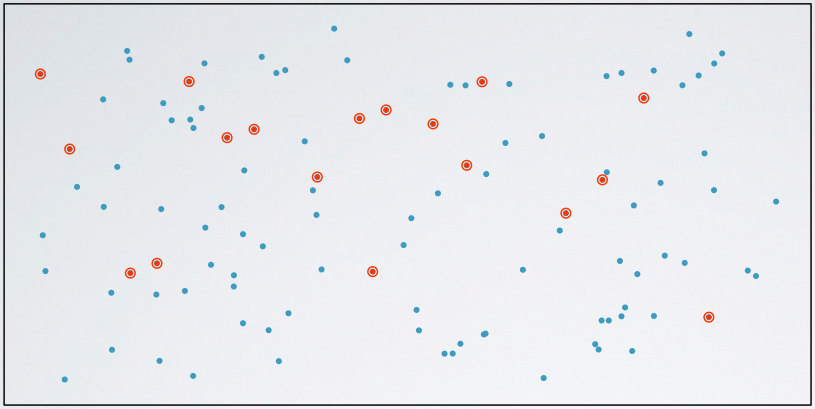
\includegraphics[width=0.9\textwidth]{Simple}
\end{center}
\end{frame}

\begin{frame}{Кластерное}
\begin{center}
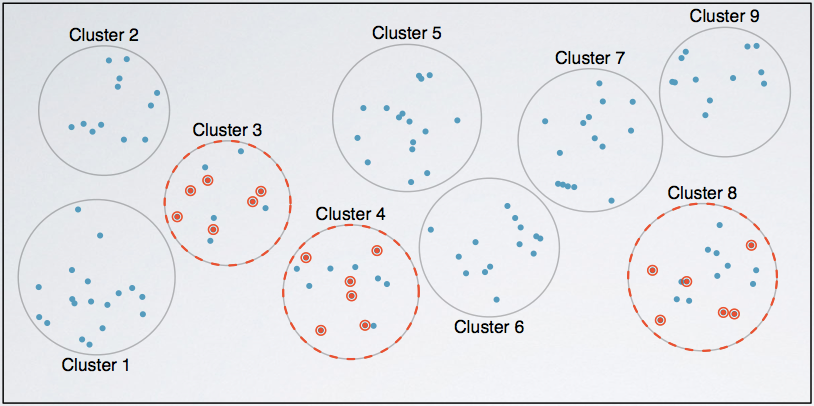
\includegraphics[width=0.9\textwidth]{Cluster}
\end{center}
\end{frame}

\begin{frame}{Стратифицированное}
\begin{center}
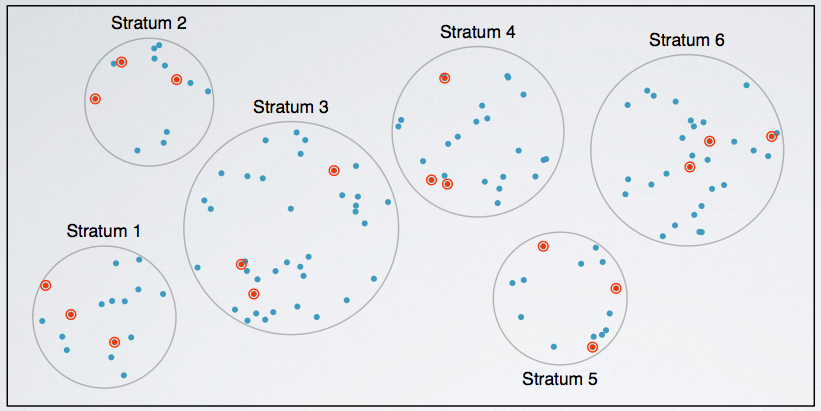
\includegraphics[width=0.9\textwidth]{Stratified}
\end{center}
\end{frame}

\begin{frame}{Как выбрать нужное?}
Надо учитывать:
\begin{itemize}
   \item природа и размер возможного сэмпла;
   \item наличие дополнительной информации об элементах;
   \item необходимая точность измерений;
   \item точность отдельных измерений в сэмплировании;
   \item стоимость измерений.
\end{itemize}
\end{frame}

\subsection{О чем еще надо подумать при создании обучающей выборки}
\begin{frame}{Как делать не нужно}{Байки про ошибки в создании обучающей выборки}
\small
\begin{itemize}
  \item Соотношение положительных и отрицательных примеров % Про LTR без фильтрации
  \item Все решения одинаково бесполезны % YLTRC T1 identity of observation
  \item Ошибка в данных больше разницы между методами % РОМИП 2003
  \item Правда в глазах смотрящего (про ошибки в примерах) % "Моя формула не может не выигрывать у прода!"
  \item Нужно следить за распределением важных параметров, независимо от способа сбора данных % от poyarkov@
  \item Устаревшие данные % Окна с Дмитрием Нагиевым
  \item Correlation vs. Causation % от poyarkov@ 
  \item Зависимость результата от одной точки или класса точек % Надо поднять vk.com, остальные запросы не важны!
  \item Закодировать ответ в DS % Хорошей мы называем сессию, которая заканчивается кликом и что-то еще
\end{itemize}
\end{frame}

\begin{frame}{Создание DS --- тоже оптимизация}
\small
Как же понять что построенное множество хорошее? Хотим такого:
$$\begin{array}{rl}
\hat{H} =& \arg \max_{H} \mu_{\xi \sim D} T(y_{\xi}, H(x_{\xi})) \\
    =& \arg \max_{H} \mu_{\xi \sim \Gamma} T(y_{\xi}, H(x_{\xi}))
\end{array}$$
Но делать будем иначе:
$$
D = \arg \max_{D} \mu_{\eta \sim \Gamma} T(y_{\eta}, \arg \max_{H} \mu_{\xi \sim D} T(y_{\xi}, H(x_{\xi}))(x_\eta))
$$
Это такая оптимизация
\end{frame}

\begin{frame}{Заключение о построении DS}
Это все область выборочного контроля про которую много написано:\\
\textit{George E.P. Box, А. И. Орлов, В.П. Боровиков}
Создание хорошего обучающего множества --- половина успеха. У меня нету универсальной схемы как такое делать, и есть ощущение, что это на грани искусства.
\end{frame}

\section{Повторное сэмплирование}

\begin{frame}{Выборка как генеральная совокупность}
\begin{itemize}
  \item LOO методы и jackknife оценки
  \item Bootstraping подход (Монте-Карло на выборке)
  \item Слабая аксиоматика Воронцова
\end{itemize}
\end{frame}

\begin{frame}{Leave One Out}
Выберем один из примеров и посмотрим насколько поменяется выборка, если его в ней не будет. Усредним по всем.\\
\small
Эту логику можно применять например так:
\normalsize
$$
Var_{LOO}(\{x_i\}) = \frac{1}{m} \sum_{i=1}^m \left(x_i - \bar{x}_{-i}\right)^2 = \frac{1}{(m-1)^2} Var(\{x_i\})
$$

\end{frame}

\begin{frame}{Jackknife оценки}
Пускай нас интересует статистика $\theta$, $\hat{\theta}$---ее выборочная оценка и $\bar{\theta} = \frac{1}{m} \sum_i \hat{\theta}_{-i}$.
$$\begin{array}{rl}
&\mathbb{E}(\hat{\theta}) = \theta + \frac{a}{m} + \frac{b}{m^2} + O(m^{-3}) \\
\Rightarrow & \mathbb{E}(\hat{\theta} - \bar{\theta}) = \frac{a}{m(m-1)} + O(m^{-3}) \\
\Rightarrow & b_{jack} = (m-1)(\bar{\theta} - \hat{\theta})
\end{array}$$
\end{frame}

\begin{frame}{Bootstrapping}{B. Efron ``Bootstrap methods: another look at the jackknife''}
Зачем ограничиваться одним примером? Устроим на нашей ``генеральной совокупности'' Монте-Карло:
\begin{enumerate}
  \item рассматривая выборку как генеральную совокупность, породим повторную выборку $X'$
  \item вычислим интересующую нас статистику $\hat{\theta}$ на $X'$
  \item проделаем 1 и 2 достаточное количество раз и построим эмпирическое распределение $\theta$
  \item исследуем эмпирическое распределение и сделаем выводы про $\theta$
\end{enumerate}
\end{frame}

\begin{frame}{Bootstrapping: простая реализация}
\begin{enumerate}
  \item случайно отсортируем исходную выборку
  \item выбросим $i$ равномерное от $1$ до $m$
  \item возьмем $i$-й пример в новую выборку
  \item повторим п. 2 и 3 $m$ раз
  \item посчитаем на полученной выборке значение $\theta$
  \item исследуем поведение $\theta$ на порожденных выборках
\end{enumerate} 
\end{frame}

\begin{frame}{Bootstrapping: практические реализации}
К сожалению в исходной версии bootstraping часто не эффективен с точки зрения производительности \uncover<2>{(Почему?)}
\begin{itemize}
  \item Бросить много пуассонов с $\lambda = 1$
  \item Байесовский bootstrap (волшебный log)
  \item Гладкий bootstrap (шумный сигнал)
  \item etc.
\end{itemize}
\end{frame}

\begin{frame}{Несколько рекомендаций}
Когда нельзя пользоваться bootstrapping'ом:\small
\begin{itemize}
  \item Когда бесконечная дисперсия
  \item Когда совсем мало примеров и возможны повторы $X'$
\end{itemize}
\normalsize
Нужно всегда помнить что:\small
\begin{itemize}
  \item Повторные выборки зависимы и степень зависимости варьируется от $m$
  \item В повторных выборках значение, например, дисперсии часто ниже чем на генеральной совокупности
  \item Чтобы понять насколько результат смещен можно применить дополнительные деления выборки
\end{itemize}
\end{frame}

\begin{frame}{Домашнее задание}
\begin{itemize}
  \item Сгенерировать последовательность $\{(x_i, y_i)| x_i, y_i \sim U(0,1)\}_{i=1}^m$, $m=10000$
  \item Выбросить минимально возможное количество примеров так, чтобы $y$ стало линейно зависимо от $x$ c уровнем значимости $\alpha=0.05$
  \item Сообщить процент выброшенного
\end{itemize}
\end{frame}

\section{Переборные методы}

\begin{frame}{Переборные методы как частный случай сэмплирования}
Сэмплирование можно использовать не только для сбора данных! Представим себе, что процесс оптимизации устроен так:
$$
\hat{H} = \arg \max_{\beta \in \mathbb{R}^m} \mathbb{E}_{\xi \sim D}(T(y_{\xi}, H(x_{\xi}, \beta)))
$$
И нету у нас никаких способов понять свойства зависимости $T$ от $\beta$.
\end{frame}

\subsection{Формальная постановка}
\begin{frame}{Формальная постановка}
$$
\hat{H} = \arg\max_H P(H|X)
$$
\begin{description}
  \item[\color{green}+] если известны вероятности можно попробовать посэмплировать решения;
  \item[\color{red}---] не определено пространство F;
  \item[\color{red}---] неясно как устроить обход.
\end{description}
\end{frame}

\begin{frame}{Иногда все просто}
$$
\hat{H} = \arg\max_{H \in \{H_i\}_{i=1}^n} P(H|X)
$$
\begin{enumerate}
  \item введём порядок обхода;
  \item переберём все возможные решения;
  \item составим взвешенное решение/выберем лучшее.
\end{enumerate}
\end{frame}

\begin{frame}{Но чаще всё непросто}
$$
\hat{H} = \arg\max_{H \in \{H_i\}_{i=1}^\infty} P(H|X)
$$
или совем запущено:
$$
\hat{H} = \arg\max_{H(x, \beta), \beta \in \mathbb{R}^k} P(H|X)
$$

\begin{enumerate}
  \item введём порядок обхода;
  \item применим систематическое сэмплирование;
  \item составим взвешенное решение/выберем лучшее.
\end{enumerate}
\end{frame}

\subsection{Случайное блуждание}
\begin{frame}{Случайное блуждание I}
\small
$$
H = H(x, \beta), \beta \in \mathbb{R}^k
$$
Чтобы построить порядок обхода можно воспользоваться такой схемой:
$$\begin{array}{l}
H_t = H(x, \beta_t) \\
\mathcal{A} = \left\{\begin{array}{l}
\beta_{t+1} = \beta_t + \xi \\ C(\beta_{t+1} | \{\beta_i\}_0^t)
\end{array}\right.
\end{array}$$
Для этого необходимо определить:
\begin{enumerate}
  \item начальную точку $\beta_0$;
  \item способ сделать шаг $\xi$;
  \item условие принятия этого шага $C$.
\end{enumerate}
\end{frame}

\begin{frame}{Случайное блуждание II}
На что стоит обратить внимание при построении блуждания:
\begin{itemize}
  \item размерность $\beta$ может быть меньше чем кажется;
  \item ограничения на $\beta$ существенно осложняют процедуру.
\end{itemize}
\end{frame}


\begin{frame}{Некоторые виды случайного блуждания}
\begin{itemize}
  \item множество фиксированных шагов $\xi \sim U(\{\xi_i\}_1^m)$;
  \item гауссовское $\xi_t \sim N(\mu, \sigma^2)$;
  \item самозависимое (генетика, рои, etc.);
  \item etc.
\end{itemize}
\end{frame}

\subsection{Hill climbing}
\begin{frame}{Simple hill climbing}
$$\begin{array}{l}
\xi \sim U(\{\xi_i\}_1^{2k}), \xi_{i} = -1^{i~mod~2}\omega_t,\\
\\
C(\beta_{t+1}|\beta_t) = \frac{P(H(\beta_{t+1})|X)}{P(H(\beta_t)|X)} > 1 \\
\end{array}$$
Свойства:
\begin{itemize}
  \item простой;
  \item быстро сходится;
  \item зависим от выбора начальной точки;
  \item etc.
\end{itemize}
\end{frame}

\begin{frame}{Random-restart (shotgun) hill climbing}
\begin{center}
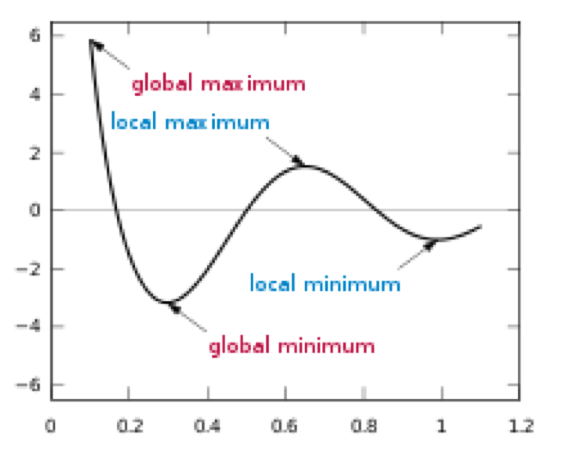
\includegraphics[width=0.4\textwidth]{hill_climb.png}
\end{center}
\footnotesize
Проблемы:
\begin{itemize}
  \item сходится в локальный максимум;
  \item может долго сходиться, если начало далеко от максимума;
  \item аллеи.
\end{itemize}
$\Rightarrow$ Можно рестартить hill climbing из разных начальных точек
\end{frame}

\subsection{Сэмплирование марковскими процессами}
\begin{frame}{Интуиция}
Мы бы хотели получить сэмплирование, а для этого:
\begin{itemize}
  \item хорошо бы обойти всё пространство;
  \item нельзя всегда ходить ''по шерсти'';
  \item скорость движения должна меняться в зависимости от плотности.
\end{itemize}
$\Rightarrow$ Markov Chain Monte-Carlo (MCMC)
\end{frame}

\begin{frame}{Metropolis-Hastings алгоритм}

Введем $p(\beta_1|\beta_2)$, отвечающую за локальность.
$$\begin{array}{l}
\alpha = \frac{P(H_{\beta_{t+1}}|X)P(\beta_{t+1}|\beta_t)}{P(H_{\beta_t}|X)P(\beta_t|\beta_{t+1})}\\
\\
\psi \sim U(0,1)\\
\\
C(\beta_{t+1}|\beta_t) = \left\{  
           \begin{array}{ll}  
            1,& \alpha \ge \psi \\  
            0 &\\  
           \end{array}   
           \right.  
\end{array}$$
Например, $P(\beta_{t+1}|\beta_t) \sim N(\beta_t,\sigma^2E)$ \\
Если $P(\beta_1 | \beta_2) = P(\beta_2 | \beta_1)$ --- это Metropolis \\ 
\end{frame}

\begin{frame}{Свойства}
\begin{center}
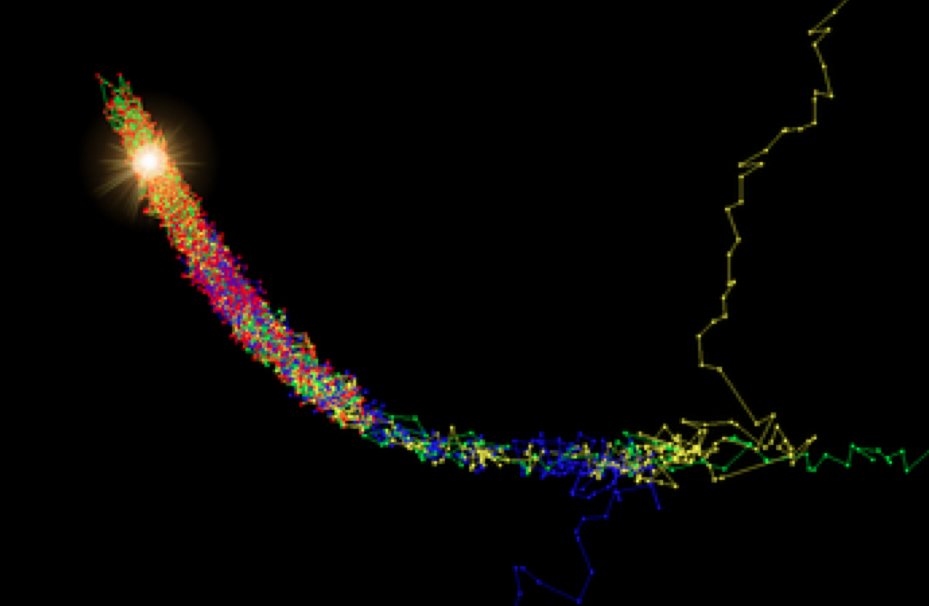
\includegraphics[width=0.5\textwidth]{mcmc.png}
\end{center}
\footnotesize
\begin{description}
  \item[\color{green}+] Обходит всё пространство
  \item[\color{green}+] Это действительно взвешенное сэмплирование
  \item[\color{red}---] Последовательные самплы похожи друг на друга
  \item[\color{red}---] На этапе разогрева показывает что-то странное
\end{description}
$\Rightarrow$ \textit{Точно придём в максимум!} \\
\end{frame}

\begin{frame}{Свойства}
\begin{center}
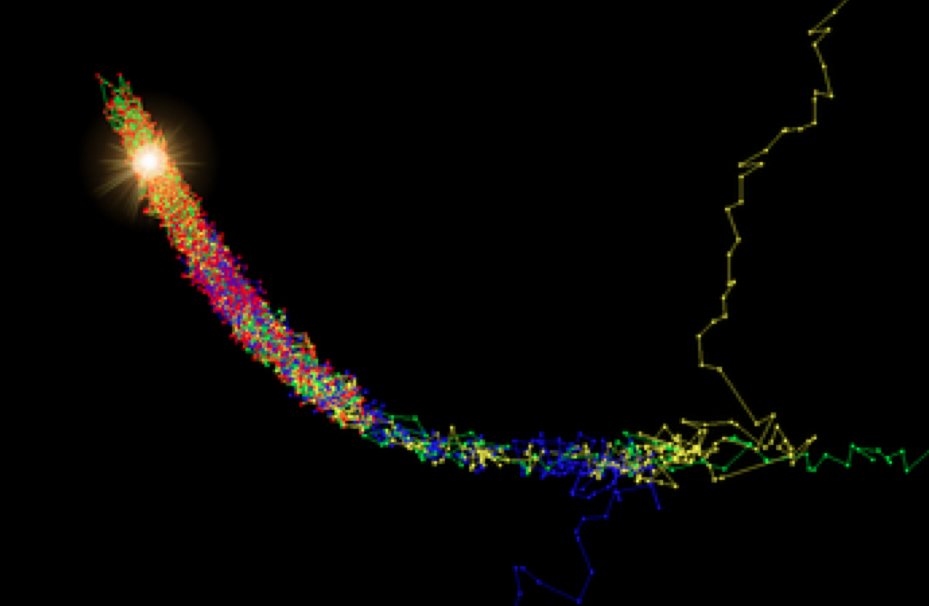
\includegraphics[width=0.5\textwidth]{mcmc.png}
\end{center}
\footnotesize
\begin{description}
  \item[\color{green}+] Обходит всё пространство
  \item[\color{green}+] Это действительно взвешенное сэмплирование
  \item[\color{red}---] Последовательные самплы похожи друг на друга
  \item[\color{red}---] На этапе разогрева показывает что-то странное
\end{description}
$\Rightarrow$ \textit{Точно придём в максимум!} \\
\textbf{Проблема только с тем, что придём за бесконечное время}
\end{frame}

\begin{frame}{Сложности в использовании}
\begin{itemize}
  \item Сходимость зависит от выбора $P(\beta_{t+1}|\beta_{t})$
  \item Если хотим использовать разумное распределение, оно многомерное $\Rightarrow$ его сложно реализовывать
\end{itemize}
\end{frame}

\subsection{Expectation-Maximization}
\begin{frame}{Пример с дартс I}
\small
Вася и Петя повесели на стене мишень и поиграли в дартс. На следующий день пришел их бригадир Юра и задался вопросом кто из подчиненных будет заделывать дырки в стенах.
\begin{itemize}
  \item Будет честнее, чтобы ``косой'' платил больше
  \item Дырки все одинаковые
  \item Каждый говорит: ``да я токо разок кинул!''
  \item Один признался, что: ``ну вот это --- моя дырка''
  \item Играли без употребления, так что можно считать, что кидали $\sim N(m_i, \Sigma_i), i \in$ \{Вася, Петя\} и параметры не менялись во времени
\end{itemize}
\textbf{Надо помочь Юре!}
\end{frame}

\begin{frame}{Пример с дартс II}
\small
При фиксированных параметрах вероятность увидеть дырки $\{x_j\}, x_j \in \mathbb{R}^2$
$$
LL = \sum_j \log(\pi N(m_A, \Sigma_A)(x_j) + (1 - \pi) N(m_B, \Sigma_B)(x_j))
$$
где $A$ --- Вася, $B$ --- Петя, $\pi$ --- доля Васиных бросков, $m_i$ --- сбитость прицела, $\Sigma_i$ --- разброс стрелка. \\
Максимизировать такое добро трудновато из-за суммы под логарифмом. Было бы классно точно знать, что тот или иной бросок точно сделал Вася $A_t \in \{0,1\}$:
$$
LL = \sum_t A_t \log(N(m_A, \Sigma_A)(x_j)) +  (1 - A_t) \log(N(m_B, \Sigma_B)(x_j))
$$
В таком варианте все совсем просто считается (если мы еще не забыли формулу плотности нормального многомерного распределения :))
\end{frame}

\begin{frame}{Пример с дартс III}
\small
Если чуть более формально, то мы ввели скрытую/ненаблюдаемую переменную $I(A)$ (такое называется data augmentation) и хотим:
\begin{enumerate}
  \item Прикинуть начальные $m_i, \Sigma_i, \pi$
  \item Посчитать ожидание скрытого параметра $A_j = \mu({(m_i, \Sigma_i}, \pi)$
  \item В условиях найденных $A_j$ максимизировать $LL$
  \item Перейти к второму шагу до сходимости
\end{enumerate}
\end{frame}

\begin{frame}{Expectation maximization алгоритм}
\small
Фокус, который мы проделали называется $EM$-алгоритм. Пускай данные у нас состоят из видимой части $L$ и скрытой $Z$, $X = (L,Z)$. Мы хотим найти оптимальные параметры $\beta$:
$$
log P(L|\beta)) = log P(X|\beta)
$$
\begin{enumerate}
  \item Возьмем какой-то $\beta_0$
  \item Посчитаем ожидание (expectation step):
  $$
  \mathbb{E}(\beta | \beta_t) = \mathbb{E}_Z \left(log P(X, \beta, Z | \beta_t \right))
  $$
  \item Проведем оптимизацию (maximization step):
  $$
  \beta_{t+1} = \arg \max_{\beta} \mathbb{E}(\beta | \beta_t)
  $$
  \item Перейти к второму шагу до сходимости
\end{enumerate}
\end{frame}

\subsection{Сэмплирование Гиббса как расширение EM}

\begin{frame}{Немного про Гиббса/Больцмана}
Есть такое распределение:
$$
p(x) = \frac{e^\frac{e(x)}{kT}}{Z = \int_x e^\frac{e(x)}{kT} dx}
$$
Про него известно, для фиксированной функции $e(x) \ge 0: Z < \infty$ и условии на общую энергию системы:
$$
\int_x e(x) dP(x) \le const
$$
оно доставляет в максимум энтропию. А еще это добро эквивалентно MRF.
\end{frame}
\begin{frame}{Алгоритм Гиббса}
В Метрополисе есть проблема: многомерное распределение $P(H|X) = P(\beta|X)$. Можно попробовать рассматривать его по частям.
\begin{enumerate}
  \item Начнем с какого-то $\beta$
  \item Сгенерируем $\beta_{t+1}$ по правилам
$$
P(\beta_{t + 1,i} | X, \beta_{t+1,1},\ldots,\beta_{t+1, i-1}, \beta_{t, i+1},\ldots, \beta_{t,n})
$$
  \item Будем бегать по $i=1\ldots n$, пока не сойдется
  \item Полученная $\beta$ --- следующая точка сэмплирования
  \item Пока хочется идем в п.2
\end{enumerate}
\end{frame}

\begin{frame}{Пример с дартс IV}
\small
На языке товарищей Геман:
\begin{enumerate}
  \item Прикинуть начальные $m_i, \Sigma_i, \pi$
  \item Для каждого сампла сгенерировать $A_j$ из текущего $\pi$
  \item В условиях найденных $A_j$ максимизировать $LL$
  \item Перейти к второму шагу до сходимости того момента пока распределение параметров не перестанет меняться
\end{enumerate}
\end{frame}

\begin{frame}{Как можно построить $P(F|X)$ для RMSE}
$$\begin{array}{l}
P(\beta|X) = \frac{e^{-c\|H(\beta|X) - Y\|_2}}{Z} \\
\\
Z = \int\limits_{\beta} e^{-c\|H(\beta|X) - Y\|}d\beta
\end{array}$$
Если максимизируем, то надеемся задрать $Y$ так, чтообы $Z$ был определён. 

Есть только одна проблема: \uncover<2->{мы хотим максимизировать, а не считать среднее :)}
\end{frame}

\begin{frame}{NFL: формальная формулировка}
$$\begin{array}{rl}
d_m =& \{(d^x_m(1), d^y_m(1)), \ldots, (d^x_m(m), d^y_m(m))\} \\
f: & \mathcal{X} \to \mathcal{Y} \\
\mathcal{F}= & \mathcal{Y}^\mathcal{X} \\
p(f) = & \frac{1}{\mathcal{F}} ёё
\end{array}$$

\begin{theorem}[David Wolpert and William G. Macready (1997)]
Для любых двух способов обхода $a_1$ и $a_2$:
$$\begin{array}{rl}
\sum_f P(d^y_m|f,m,a_1) = \sum_f P(d^y_m|f,m,a_2)
% \sum_f p(d^y_m|f_0,M,m,a_1) = \sum_f p(d^y_m|f_0,M,m,a_2)
\end{array}$$
\end{theorem}
\end{frame}

\begin{frame}{NFL: следствия}
\begin{itemize}
  \item Нам всем хватит работы :)
  \item Полоса белая, полоса черная
  \item Нужно искать близкие задачи
\end{itemize}
\end{frame}

\section{Заключение}
\begin{frame}{Заключение}
Сэмплирование очень полезная вещь:
\begin{itemize}
  \item собирать данные;
  \item брать интегралы;
  \item обучаться.
\end{itemize}
Посмотрите на bayesian inference и библиотеку Гиббса для него: BUGS.
\end{frame}

\begin{frame}{Задание на дом}
\begin{itemize}
  \item Датасет, как обычно, в svn
  \item Суть - учимся предсказывать размер аудитории сервиса
  \item $N(t) = (\frac{1}{1 + e^{at+b}})N_0$
  \item Ищем $a$, $b$, $N_0$
  \item Можно прямо hill climbing
  \item Можно подумать и воспользоваться алгоритмом Гиббса (это будет плюсом)
  \item Дедлайн 17 октября
\end{itemize}
\end{frame}

\end{document}
